% !TEX root = ../main.tex

\chapter{图表、公式格式}

\section{图表格式}
\begin{figure}[!htp]
  \centering
  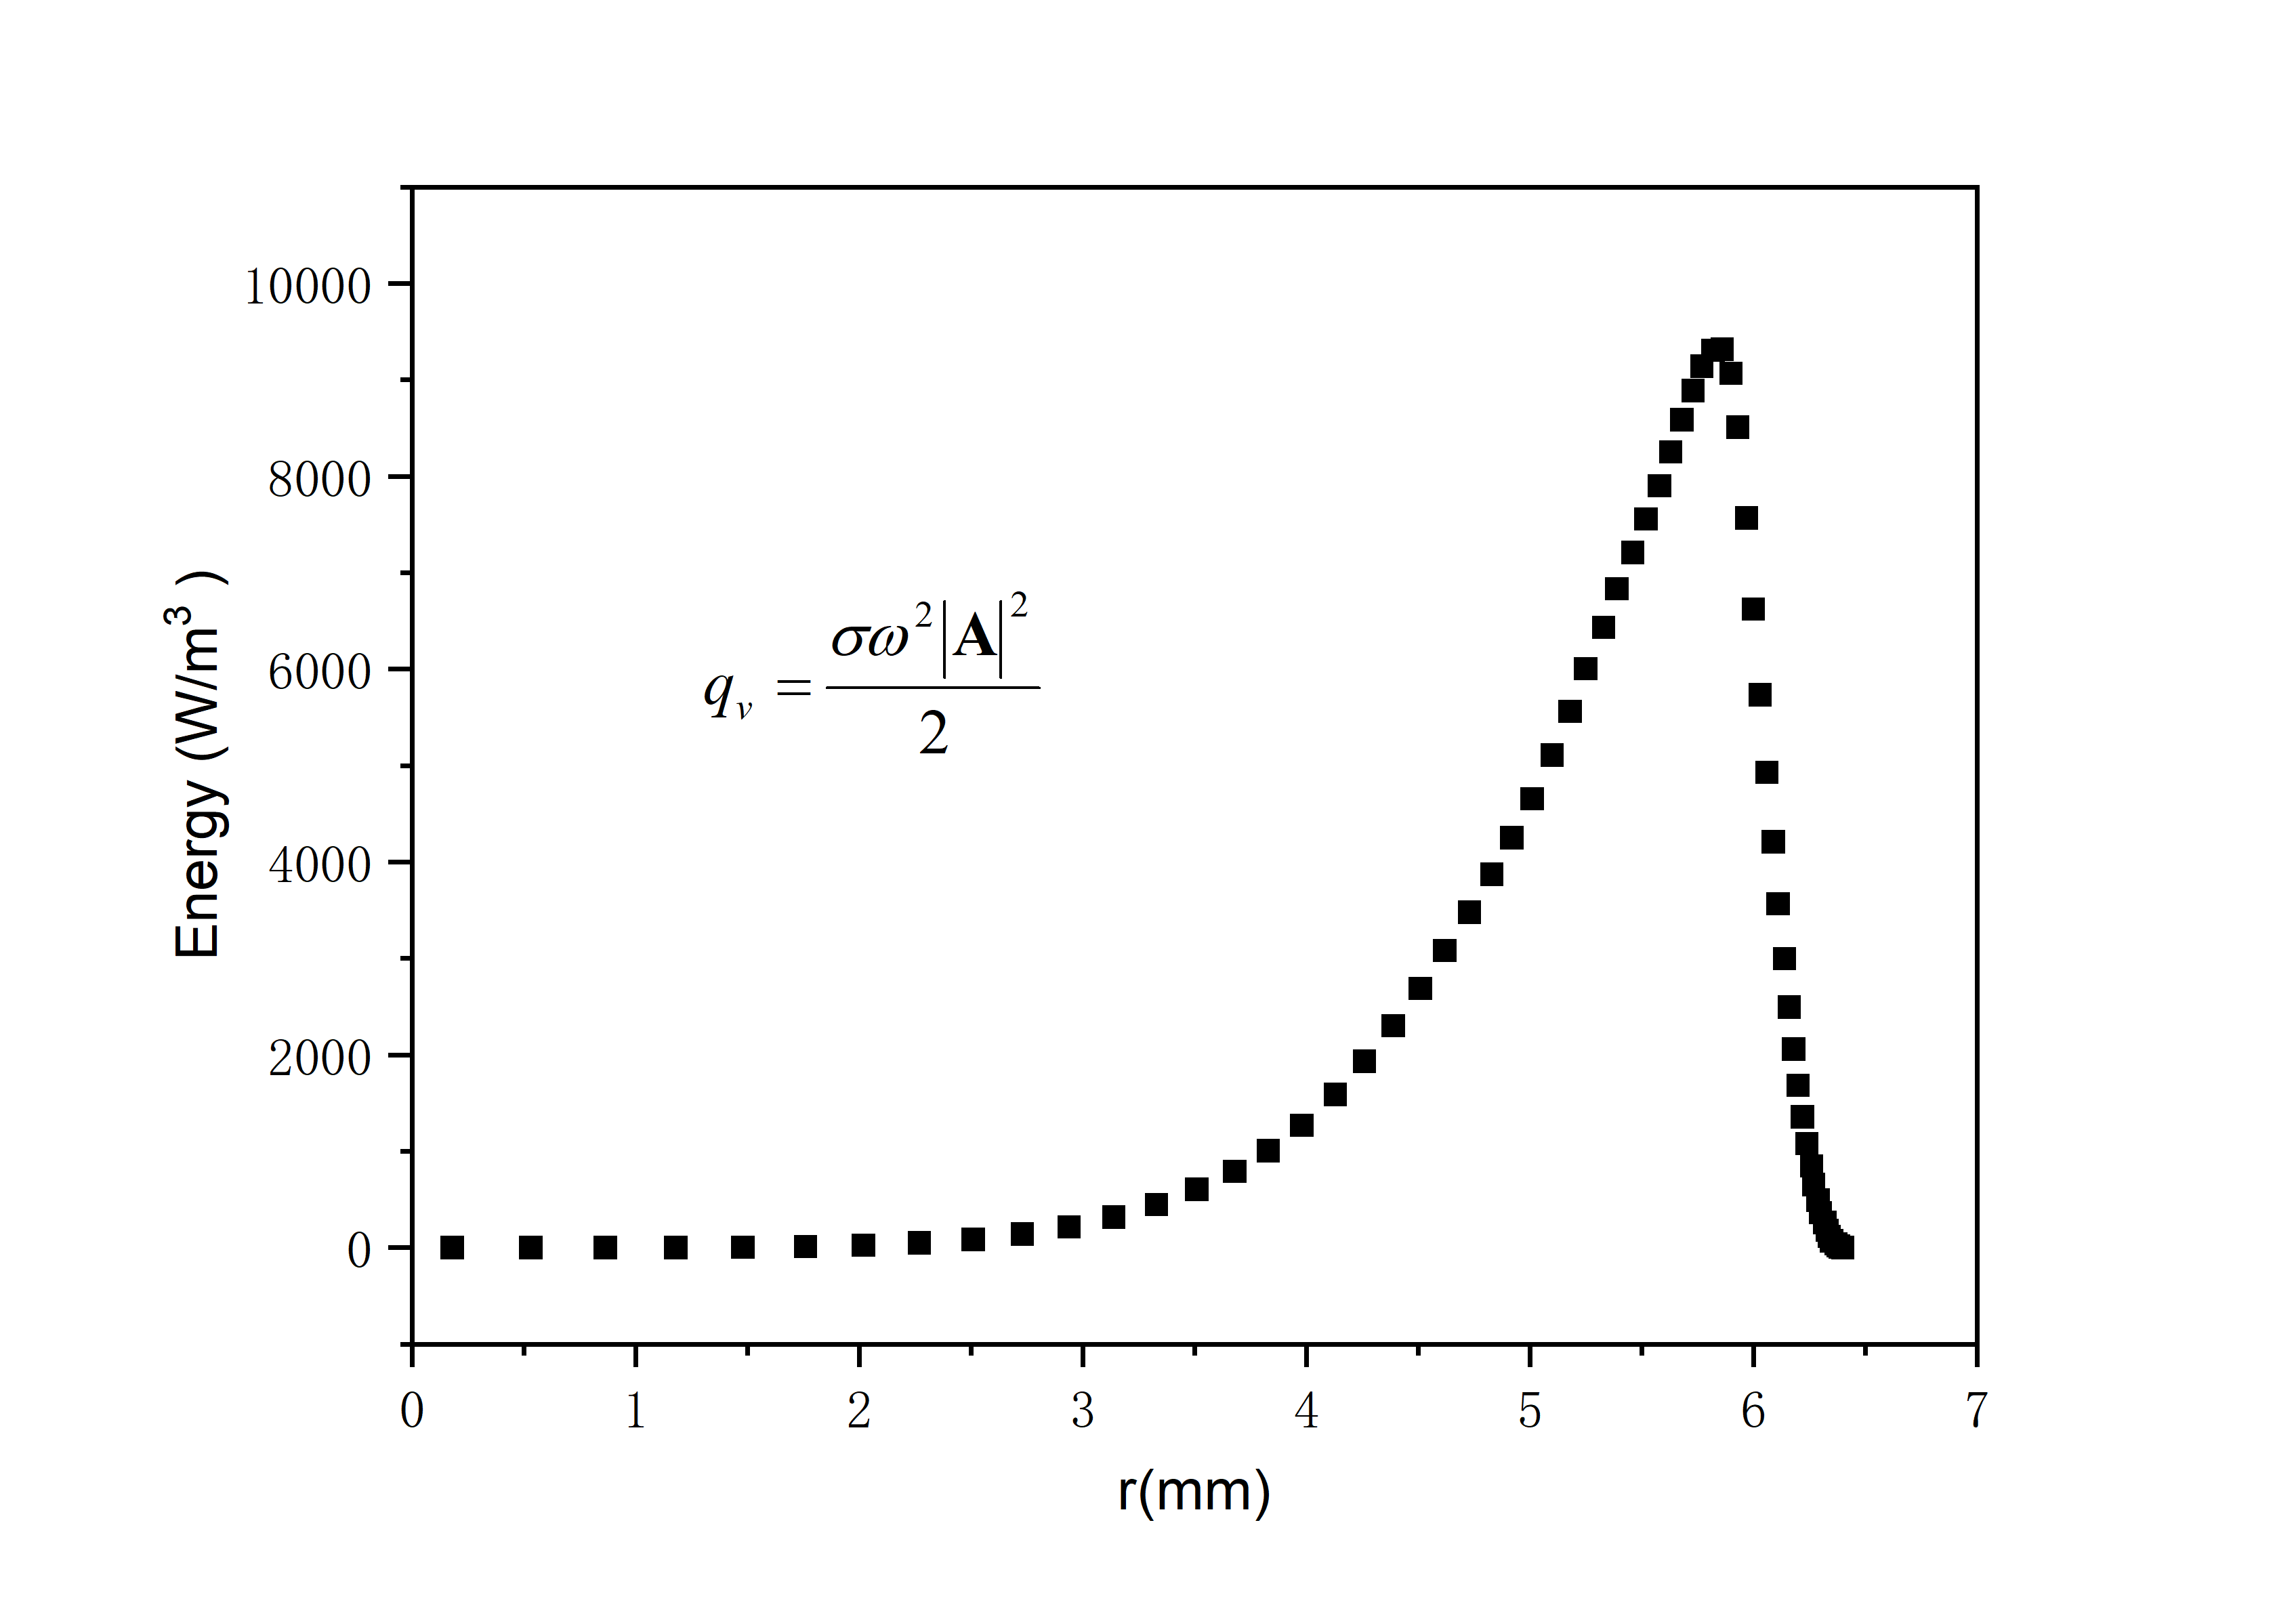
\includegraphics[width=8cm]{figures/energy.png} 
  \caption{内热源沿径向的分布}
  \label{fig:energy}
\end{figure}

\begin{figure}[!hbtp]
  \centering
  \subcaptionbox{健康/损伤信号}%
                [7cm]{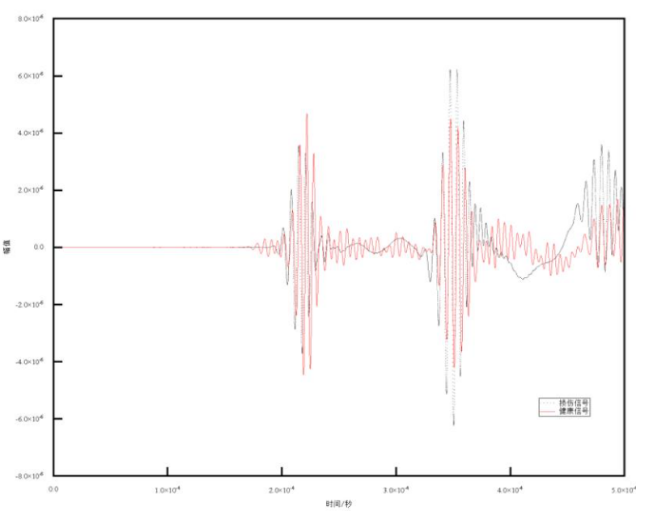
\includegraphics[height=6cm]{figures/signal_1.png}}
  \hspace{1cm}
  \subcaptionbox{散射信号}%
                [7cm]{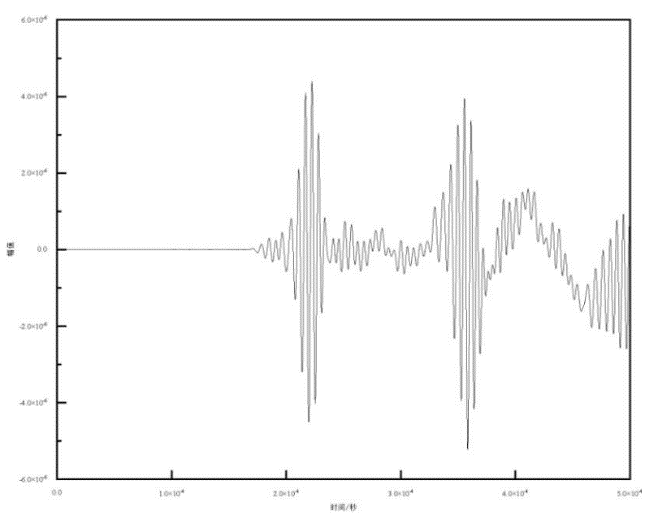
\includegraphics[height=6cm]{figures/signal_2.png}}
  \caption{响应信号处理}
  \label{fig:bisubcaptionbox}
\end{figure}

\begin{ThreePartTable}
  \begin{longtable}[c]{*{4}{c}}
    \caption{高频感应加热的基本参数}
    \label{tab:data} \\
    \toprule
     \multicolumn{1}{c}{感应频率} & \multicolumn{1}{c}{感应发生器功率}
      & \multicolumn{1}{c}{工件移动速度} & \multicolumn{1}{c}{感应圈与零件间隙}
    & \multicolumn{1}{c}{(kHz)} & \multicolumn{1}{c}{(\% ×80kW)}
    & \multicolumn{1}{c}{(mm/min)} & \multicolumn{1}{c}{(mm)}\\
    \midrule
    \endfirsthead
    \multicolumn{4}{l}{\textbf{续表~\thetable}} \\
    \toprule
     \multicolumn{1}{c}{感应频率} & \multicolumn{1}{c}{感应发生器功率}
      & \multicolumn{1}{c}{工件移动速度} & \multicolumn{1}{c}{感应圈与零件间隙}
    & \multicolumn{1}{c}{(kHz)} & \multicolumn{1}{c}{(\% ×80kW)}
    & \multicolumn{1}{c}{(mm/min)} & \multicolumn{1}{c}{(mm)}\\
    \midrule
    \endhead
    \hline
    \multicolumn{4}{r}{}
    \endfoot
    \endlastfoot
    250	& 88 & 5900	& 1.65 \\
    250	& 88 & 5900	& 1.65 \\
    250	& 88 & 5900	& 1.65 \\
    250	& 88 & 5900	& 1.65 \\
    250	& 88 & 5900	& 1.65 \\
    250	& 88 & 5900	& 1.65 \\
    250	& 88 & 5900	& 1.65 \\
    250	& 88 & 5900	& 1.65 \\
    250	& 88 & 5900	& 1.65 \\
    250	& 88 & 5900	& 1.65 \\
    250	& 88 & 5900	& 1.65 \\
    250	& 88 & 5900	& 1.65 \\
    250	& 88 & 5900	& 1.65 \\
    250	& 88 & 5900	& 1.65 \\
    250	& 88 & 5900	& 1.65 \\
    250	& 88 & 5900	& 1.65 \\
    250	& 88 & 5900	& 1.65 \\
    250	& 88 & 5900	& 1.65 \\
    250	& 88 & 5900	& 1.65 \\
    250	& 88 & 5900	& 1.65 \\
    250	& 88 & 5900	& 1.65 \\
    250	& 88 & 5900	& 1.65 \\
    250	& 88 & 5900	& 1.65 \\
    250	& 88 & 5900	& 1.65 \\
    250	& 88 & 5900	& 1.65 \\
    250	& 88 & 5900	& 1.65 \\
    250	& 88 & 5900	& 1.65 \\
    250	& 88 & 5900	& 1.65 \\
    250	& 88 & 5900	& 1.65 \\
    250	& 88 & 5900	& 1.65 \\
    250	& 88 & 5900	& 1.65 \\
    250	& 88 & 5900	& 1.65 \\
    250	& 88 & 5900	& 1.65 \\
    250	& 88 & 5900	& 1.65 \\
    250	& 88 & 5900	& 1.65 \\
    250	& 88 & 5900	& 1.65 \\
    250	& 88 & 5900	& 1.65 \\
    250	& 88 & 5900	& 1.65 \\
    250	& 88 & 5900	& 1.65 \\
    250	& 88 & 5900	& 1.65 \\
    250	& 88 & 5900	& 1.65 \\
    250	& 88 & 5900	& 1.65 \\
    250	& 88 & 5900	& 1.65 \\
    \bottomrule
  \end{longtable}
\end{ThreePartTable}

\section{公式格式}
\begin{equation}
 \frac{1}{\mu} \nabla^{2} \mathbf{A}-j \omega \sigma \mathbf{A}-\nabla\left(\frac{1}{\mu}\right) \times(\nabla \times \mathbf{A})+\mathbf{J}_{0}=0
\end{equation}


\section{本章小结}
本章介绍了……
